%%This is a very basic article template.
%%There is just one section and two subsections.
\documentclass[11pt]{book}

\usepackage{graphicx}
\usepackage{rotating}

\usepackage{fourier}
\usepackage[T1]{fontenc}

\usepackage{xspace}
\usepackage[hyperindex=true, bookmarks=true,
            pdftitle={MMTk},
            pdfauthor={Robin Garner},
            colorlinks=false,
            pdfborder=0,
            pagebackref=true,
            citecolor=blue,
            plainpages=false,
            pdfpagelabels,
            hyperfootnotes=false]{hyperref}
\renewcommand*{\backref}[1]{}  
   \renewcommand*{\backrefalt}[4]{
      \ifcase #1 
         (not cited)
      \or
         (cited on page #2)
      \else
         (cited on pages #2)
      \fi} 

\usepackage{subfloat}
\usepackage{subcaption}
\usepackage{caption} 


\usepackage{multirow}
\usepackage{listings}
\lstloadlanguages{java}
\lstset{basicstyle=\footnotesize\ttfamily,language=Java,numbers=left,captionpos=b,frame=single, 
aboveskip=12pt,
belowskip=12pt,
framesep=6pt,
        rulesep=4pt}

% Includes the \citet and \citep macros
\usepackage[square]{natbib}

\usepackage[obeyDraft,color=todocolor, colorinlistoftodos]{todonotes}

\usepackage{tikz}
\usepackage{tikzuml/tikz-uml}

\input{macros}

\begin{document}

\part{Introduction}

% Intro
\input{intro}

% High level outline of an MMTk plan.  
% - How allocation works
% - How collection works
% - Design criteria and constraints
%   - Thread-local versus global
%   - Inlining
\chapter{Memory Management in MMTk}

As an automatic memory manager, \mmtk performs two principal functions: 
allocation of new objects, and garbage collection.  This chapter describes
how an \mmtk plan performs these operations, largely independent of the 
garbage collection algorithm used.  Where specific examples are required,
we use the mark-sweep plan, but in general the discussion should apply to all
\mmtk plans.

\section{Layout of Virtual Memory}

\mmtk one fundamental assumption about the layout of virtual memory, namely that
there is a single contiguous range of addresses that it can manage exclusively. 
Within this region (the \emph{heap}), address ranges are assigned to
\emph{spaces}, which can be either \emph{contiguous} or \emph{discontiguous}.  A
\emph{space} is a region of virtual memory that is manages according to a
\emph{policy}, for example the Large Object Space, which uses an
implementation of Baker's Treadmill.  Spaces are allocated in \emph{chunks}, of
4MB.

A fixed area of virtual memory in the lowest range managed by \mmtk\ is reserved
for the virtual machine's code and data.  The \mmtk\ heap begins imediately
above this region.

A contiguous space occupies a fixed amount of virtual memory between a start and
end address.  
One contiguous space can be defined as occupying the
high memory addresses, a feature some generational collectors use to optimize
their write barriers.  
A discontigouous space consists of a set of 4MB chunks which may
or may not be adjacent to each other.

Different layouts are applied to 32-bit and 64-bit address spaces, as shown in
Figure~\ref{fig:vm}.
In the 64-bit layout, all spaces are allocated 2TB (41 bits) of contiguous address
space.  Discontiguous spaces are not used in the 64-bit layout.

In the 32-bit layout, contiguous spaces are defined as either fixed size or
(more typically) a fraction of the available space.  
The contiguous spaces are allocated at
increasing virtual addresses starting from the lowest available addresses.
The remaining region of memory (between the end of the highest 'low' contiguous
space and the start of the 'high' space) is allocated to discontiguous spaces,
which allocate and release 4MB chunks as required.  Most spaces in the existing \mmtk plans are discontiguous.

Mapping a virtual address to its managing space is a performance critical
operation.  In the inner loop of the transitive closure, \mmtk\ must examine
each object reference and dispatch to the \lstinline|traceObject| method of the
space that manages it.  For a contiguous space, one or two comparisons are
sufficient, but for a discontiguous space the operation requires a table lookup.

\begin{figure}[htb]
\vspace*{2ex}
\begin{minipage}{.45\textwidth}
\input{vm-layout-32-dia}
\subcaption{32-bit layout}
\end{minipage}
\hfill
\begin{minipage}{.45\textwidth}
\input{vm-layout-64-dia}
\subcaption{64-bit layout}
\end{minipage}
\caption{Virtual memory layout in 32- and 64-bit address spaces.  Actual
addresses used in the 32-bit example are configurable at build time.}
\label{fig:vm}
\end{figure}

\section{Structure of a Plan}

An \mmtk Plan is required to provide 4 classes, as described in
Section~\ref{sec:intro:plans}.
They are required to be in a separate package in the \lstinline|org.mmtk.plan|
hierarchy, have consistent names which start with the same prefix and have a
suffix that indicates which class it inherits from.
In addition, every plan that traces the heap will also define an instance of
TraceLocal, but there is more naming flexibility with this class.
In the case of the MarkSweep plan, the base name is "MS", and the 5 classes
are:
\begin{itemize}
\item \textbf{MS} - this is a singleton class that is a subclass of
\lstinline|org.mmtk.plan.Plan|.
This class encapsulates data structures that are shared among multiple threads.
\item \textbf{MSMutator} - subclass of \lstinline|org.mmtk.plan.MutatorContext|. 
This class encapsulates data structures that are local to a single mutator thread.  
In the case of Jikes RVM, a Thread is actually a subclass of this class for efficiency reasons.
\item \textbf{MSCollector} - subclass of
\lstinline|org.mmtk.plan.CollectorContext|.
This provides thread-local data structures specific to a garbage collector thread.
\item \textbf{MSConstraints} - subclass of
\lstinline|org.mmtk.plan.PlanConstraints|.
This provides configuration information that the host virtual machine might need.  
It is separated out from the Plan class in order to prevent circular class loading dependencies.
\item \textbf{MSTraceLocal} - subclass of \lstinline|org.mmtk.plan.TraceLocal|. 
This provides thread-local data structures specific to a particular way of traversing the heap.  
In a simple collector like MarkSweep, there is only one of these classes, 
but in more complex collectors there may be several.  For example, in a generational collector, 
there will be one TraceLocal class for a nursery collection, and another for a full-heap collection.
\end{itemize}

A policy is implemented
by an instance of the \lstinline|Space| class, and it is in the policy class
that the mechanics of a particular mechanism (like mark-sweep) is implemented.  
The task of a plan is to create the policy (Space) objects that manage the heap, 
and to integrate them into the \mmtk framework.  
\mmtk exposes some of this memory management policy to the host VM, 
by allowing the VM to specify an allocator 
(represented by a small integer) when allocating space.  
The interface exposed to the VM allows it to choose whether an object 
will move during collection or not, whether the object is 
large enough to require special handling \etc.  
The \mmtk plan is free (within the semantic guarantees exposed to the VM) 
to direct each of these allocators to a particular policy.

All \mmtk plans share a number of features, such as a space where the host
virtual machine's code and data lives (the \emph{vm} space), an \emph{immortal}
space where the VM can create objects that will never die, spaces for allocation
of code etc., and these common spaces are created by the Plan class.  All
``stop-the-world'' collectors share a common structure, where mutator threads are quiesced, 
mutator stacks are scanned for roots, collection occurs and the
mutators are resumed.  This basic structure is provided to \mmtk plans by
inheritance.  In the case of mark-sweep, the inheritance hierarchy of the plan
is shown in Figure~\ref{fig:gc:inheritance}.

\begin{sidewaysfigure}
\begin{center}
%\resizebox{\textwidth}{!}{%
\begin{tikzpicture}

\newcommand*{\planRow}{-0}
\newcommand*{\parRow}{-2}
\newcommand*{\simpleRow}{-4}
\newcommand*{\stwRow}{-6}
\newcommand*{\msRow}{-9}

\newcommand*{\planCol}{+1}
\newcommand*{\mutCol}{+8}
\newcommand*{\collCol}{+12}
\newcommand*{\conCol}{+4.5}
\newcommand*{\traceCol}{+16}

\begin{umlpackage}{{org.mmtk.}plan}
\umlclass[y=\planRow,x=\planCol]{Plan}{
}{}
\umlclass[y=\simpleRow,x=\planCol]{Simple}{
}{}
\umlclass[y=\stwRow,x=\planCol]{StopTheWorld}{
}{}

\umlclass[y=\planRow,x=\mutCol]{MutatorContext}{
}{}
\umlclass[y=\simpleRow,x=\mutCol]{SimpleMutator}{
}{}
\umlclass[y=\stwRow,x=\mutCol]{{S.T.W.}Mutator}{
}{}

\umlclass[y=\planRow,x=\collCol]{CollectorContext}{
}{}
\umlclass[y=\parRow,x=\collCol]{ParallelCollector}{
}{}
\umlclass[y=\simpleRow,x=\collCol]{SimpleCollector}{
}{}
\umlclass[y=\stwRow,x=\collCol]{{S.T.W.}Collector}{
}{}

\umlclass[y=\planRow,x=\conCol]{PlanConstraints}{
}{}
\umlclass[y=\simpleRow,x=\conCol]{SimpleConstraints}{
}{}
\umlclass[y=\stwRow,x=\conCol]{{S.T.W.}Constraints}{
}{}

\umlemptyclass[y=\planRow,x=\traceCol,type=abstract]{TransitiveClosure}{
}{}
\umlclass[y=\parRow,x=\traceCol]{TraceLocal}{
}{}

\begin{umlpackage}{{{org.mmtk.}plan.}marksweep}
\umlclass[y=\msRow,x=\planCol]{MS}{
}{}
\umlclass[y=\msRow,x=\mutCol]{MSMutator}{
}{}
\umlclass[y=\msRow,x=\collCol]{MSCollector}{
}{}
\umlclass[y=\msRow,x=\conCol]{MSConstraints}{
}{}
\umlclass[y=\msRow,x=\traceCol]{MSTraceLocal}{
}{}
\end{umlpackage}
\end{umlpackage}

\umlinherit[geometry=-|]{Simple}{Plan}
\umlinherit[geometry=-|]{StopTheWorld}{Simple}
\umlinherit[geometry=-|]{MS}{StopTheWorld}

\umlinherit[geometry=-|]{SimpleMutator}{MutatorContext}
\umlinherit[geometry=-|]{{S.T.W.}Mutator}{SimpleMutator}
\umlinherit[geometry=-|]{MSMutator}{{S.T.W.}Mutator}

\umlinherit[geometry=-|]{ParallelCollector}{CollectorContext}
\umlinherit[geometry=-|]{SimpleCollector}{ParallelCollector}
\umlinherit[geometry=-|]{{S.T.W.}Collector}{SimpleCollector}
\umlinherit[geometry=-|]{MSCollector}{{S.T.W.}Collector}

\umlinherit[geometry=-|]{SimpleConstraints}{PlanConstraints}
\umlinherit[geometry=-|]{{S.T.W.}Constraints}{SimpleConstraints}
\umlinherit[geometry=-|]{MSConstraints}{{S.T.W.}Constraints}

\umlinherit[geometry=-|]{TraceLocal}{TransitiveClosure}
\umlinherit[geometry=-|]{MSTraceLocal}{TraceLocal}

\umlassoc[geometry=-|,mult1={1},pos1=0.8,mult2={1..1},pos2=0.1]{Plan}{PlanConstraints}

\end{tikzpicture}

%
%}
\end{center}
\caption{Inheritance hierarchy of the mark-sweep plan.}
\label{fig:gc:inheritance}
\end{sidewaysfigure}

\subsection{Policies}

\begin{sidewaysfigure}
\include{policy-uml}
\caption{Class relations between plans and policies.  The diagram shows a
subset of the relationships, illustrating two spaces: the small code space,
defined in the Plan for all MMTk plans, and the main mark-sweep space.}
\label{fig:gc:policy-uml}
\end{sidewaysfigure}

A policy describes how a range of virtual address space is managed.  
The base class of all policies is \lstinline|org.mmtk.policy.Space|, and a
particular instance of a policy is known generically as a \emph{space}.  
The static initializer of a Plan and its subclasses define the spaces that 
make up an MMTk plan.  The relationships between the classes of a Plan and a
Policy are shown in Figure~{\ref{fig:gc:policy-uml}}.
 
\begin{lstlisting}[name=MS.java,caption=\lstname: definition of the mark-sweep
space, label=fig:gc:ms-space]
public static final MarkSweepSpace msSpace 
  = new MarkSweepSpace("ms", VMRequest.create());
public static final int MARK_SWEEP = msSpace.getDescriptor();
\end{lstlisting}

In Listing~\ref{fig:gc:ms-space}, we see the mark-sweep space defined.  Note
that we generally also define a \lstinline|static final int| space descriptor.  This is
an optimization that allows some rapid operations on spaces.

A Space is a global object, shared among multiple mutator threads.  
Each policy will also have one or more thread-local classes which provide unsynchronized allocation.  
These classes are subclasses of org.mmtk.utility.alloc.Allocator, and in the case of MarkSweep, 
it is called MarkSweepLocal.  Instances of MarkSweepLocal are created as 
part of a mutator context, as shown in Listing~\ref{fig:gc:ms-allocator}

\begin{lstlisting}[name=MSMutator.java,caption=\lstname: definition of the ms
allocator,label=fig:gc:ms-allocator]
protected MarkSweepLocal ms = new MarkSweepLocal(MS.msSpace);
\end{lstlisting}
The design pattern is that the local Allocator will allocate space 
from a thread-local buffer, and when that is exhausted it will 
acquire a lock, allocate a new buffer from the global Space, and release the lock.  
The constructor of the MarkSweepLocal class takes as a parameter the space from
which the allocator will allocate global memory.

\section{Allocation}

MMTk provides its host VM with 
two methods that it must call when allocating an object: \lstinline|alloc| which
allocates the raw memory required; and \lstinline|postAlloc|, which initializes
gc-specific fields in the object (if any).  This separation of responsibility
allows the VM some flexibility, in the rare case when it might need to
initialize an object that has been allocated by some other means (Jikes RVM
does this when building its boot image). 
These methods are implemented by the MSMutator
class in order to use fast, unsynchronized thread-local allocation before falling 
back to a slower synchronized slow-path.

The version of \lstinline|alloc| implemented in MarkSweep is shown in
Listing~\ref{fig:gc:ms-alloc}.
\begin{lstlisting}[name=MSMutator.java,
caption=\lstname: The alloc method in the mark-sweep plan.,label=fig:gc:ms-alloc] 
public Address alloc(int bytes, int align, 
                     int offset, int allocator, int site) {
  if (allocator == MS.ALLOC_DEFAULT) 
    return ms.alloc(bytes, align, offset);
  return super.alloc(bytes, align, offset, allocator, site);
}
\end{lstlisting}
The basic structure of this method is common to all MMTk plans.  
First they decide whether the operation applies to this level of abstraction 
(line 2), and if so, delegate to the
appropriate object, otherwise pass it up the chain of inheritance to the
super-class.
In the case of mark-sweep, MSMutator delegates the allocation to its
thread-local MarkSweepLocal object \lstinline|ms|.

The alloc method of MarkSweepLocal is inherited from SegregatedFreeListLocal 
(mark-sweep is not the only policy built on free-list allocation), and is shown
in Listing~\ref{fig:gc:freelist-alloc}.
\begin{lstlisting}[name=SegregatedFreeListLocal.java,
caption=\lstname: definition of the alloc method.,label=fig:gc:freelist-alloc]
public final Address alloc(int bytes, int align, int offset) { 
  int sizeClass = getSizeClass(bytes);
  Address cell = freeList.get(sizeClass);
  if (!cell.isZero()) {
    freeList.set(sizeClass, cell.loadAddress());
    cell.store(Address.zero()); // Clear the free list link
    return cell;
  }
  return allocSlow(bytes, align, offset);
}
\end{lstlisting}
This is a standard pattern for thread-local allocation: 
first we look in the thread-local space (line 3), 
and if successful return the result (lines 4-8), zeroing out the free list link
so that the object is initialized to zeros.
The instance field \lstinline|freeList| is an \lstinline|AddressArray|,
essentially an array of addresses, each of which points to a linked list of
free cells of a single size class.  Line 5 of the listing updates the
appropriate \lstinline|freeList| element to point to the next cell in the list.

If unsuccessful, we request space from the global policy via the method
\lstinline|allocSlow|, inherited from the \lstinline|Allocator| class.
This is the common interface that all allocators use to request space from the global policy.  
This will eventually call the allocator-specific \lstinline|allocSlowOnce|
method.
The workings of the \lstinline|allocSlowOnce| method are very policy-specific, 
so not appropriate to look at at this stage, but eventually all policies will 
attempt to acquire fresh virtual memory via the \lstinline|Space.acquire|
method.

\lstinline|Space.acquire| is the only correct way for a policy to allocate new
virtual memory for its own use.  The logic of \lstinline|Space.acquire| is:
\begin{lstlisting}[name=Space.java,caption=\lstname: acquiring new
pages.,label=fig:gc:space-acquire]
public final Address acquire(int pages) {
  pr.reservePages(pages);
  // Poll, either updating budget or requiring GC
  if (VM.activePlan.global().poll(false, this)) {
    VM.collection.blockForGC();
    // GC has completed, return zero to trigger retry
    return Address.zero(); 
  }
  // Page budget is ok, try to acquire virtual memory
  Address rtn = pr.getNewPages(pagesReserved, pages, zeroed);
  if (rtn.isZero()) {  
    // Failed, so force a GC
    VM.activePlan.global().poll(true, this);
    VM.collection.blockForGC();
    return Address.zero();
  }
  return rtn;
}
\end{lstlisting}

First, poll the plan to find out whether the heap is full
(Listing~\ref{fig:gc:space-acquire}, lines 2--3).
This logic is performed by the Plan instance, because it is responsible for
coordinating the demands of all spaces it defines.
The \lstinline|poll| method will request a GC if required, and return
\lstinline|true| if it has done so.
Then we wait for GC if required.
If \lstinline|Plan.poll(false,...)| returns \lstinline|false| (we are within the
allowed heap size), we call \lstinline|pr.getNewPages| to allocate virtual memory.  
At this stage we can find that we have run out of virtual memory (in the
current space), and if so, we force a GC (again, by calling \lstinline|poll|).

If a GC is performed, we return zero rather than retrying locally. 
In many plans, the next allocation request will be satisfied by re-using space 
in a page that already belongs to a policy, so the post-GC allocation 
must be performed further up in the call stack.  

The retry logic is handled in \lstinline|Allocator.allocSlowInline|.
\begin{lstlisting}[name=Allocator.java, 
                   caption=\lstname: allocSlowInline,
                   label=fig:gc:freelist-allocslow]
public final Address allocSlowInline(
    int bytes, int alignment, int offset) {
  boolean emergencyCollection = false;
  while (true) {
    Address result = allocSlowOnce(bytes, alignment, offset);
    if (!result.isZero())
      return result;
    if (emergencyCollection)
      VM.collection.outOfMemory();  // Throw an OOM Exception
    emergencyCollection = Plan.isEmergencyCollection();
  }
}
\end{lstlisting}
This code fragment shows the retry logic in the allocator.  We try allocating 
using \lstinline|allocSlowOnce|, which may recycle partially-used blocks and
eventually call Space.acquire.  If a GC occurred, we try again.  Eventually the plan 
will request an emergency collection which will (for example) cause 
soft references to be dropped.  If this fails we throw an OutOfMemoryError.

\section{Collection}

A garbage collection can be triggered by one of several events, usually 
because some resource has been exhausted.  The most common case is where
the heap is full, which in \java usually means that the user-defined limit
of the heap (with the \lstinline|-Xmx| command-line flag) has been exceeded.
In a generational collector a collection may be triggered because the nursery
is full, or because the space reserved for the remembered sets is full.
Other collectors such as the reference counting collector may collect simply
because a timer has elapsed, and concurrent collectors may start a concurrent
collection when the heap cas crossed a size threshold, then complete the
collection when the concurrent mark phase is complete.  Finally, a mutator
thread (in \java) may initiate a collection by calling the
\lstinline|System.gc()| method.


\subsection{Scheduling}

In a stop-the-world garbage collector like MarkSweep, the mutator threads run until memory is exhausted, then all mutator threads are suspended, the collector threads are activated, and they perform a garbage collection.  After the GC is complete, the collector threads are suspended and the mutator threads resume.  MMTk also has some support for concurrent collectors, in which one or more collector threads can be scheduled to run alongside the mutator, either exclusively or in addition to (hopefully briefer) stop-the-world phases. 

Thread scheduling in MMTk is handled by a GC controller thread, implemented in the singleton class org.mmtk.plan.ControllerCollectorContext  held in the static field Plan.controlCollectorContext. Whenever a collection is initiated, it is done by calling methods on this object.

\subsection{Initiating}

As mentioned above, every attempt to allocate fresh virtual memory calls the 
current plan's \lstinline|poll(...)| method.  This initiates a GC by calling
controlCollectorContext.request(), which in a stop-the-world collector like 
MarkSweep pauses the mutator threads and then wakes the collector threads.  
The main loop of the garbage collector is simply the \lstinline|run()| method of
ParallelCollector, shown below.

\begin{lstlisting}[name=ParallelCollector.java,caption=\lstname: the main loop of a collector
thread.,label=fig:gc:collector-run]
public void run() {
  while(true) {
    park();
    collect();
  }
}
\end{lstlisting}
The collect() method is specific to the type of collector, and in StopTheWorldCollector it looks like this

\begin{lstlisting}[name=StopTheWorldCollector.java,caption=\lstname: performing a garbage collection.,label=fig:gc:stw-collect]
public void collect() {
  Phase.beginNewPhaseStack(Phase.scheduleComplex(global().collection));
}
\end{lstlisting}

\subsection{Collector Phases}

Every garbage collection consists of a series of steps.  
Each step is either executed once (e.g. updating the mark 
state before marking the heap), or in parallel on all 
available collector threads (e.g. the parallel mark phase).  
The actual work of a step is done by the collectionPhase 
method of the global, collector or mutator class of a plan.

In early versions of MMTk, the main collection method was a template method, 
calling individual methods for each phase of the collection.  As the number 
of collectors in MMTk grew, this became unwieldy and has been 
replaced with a configurable mechanism of phases.  

The class \lstinline|org.mmtk.plan.Simple| defines the basic structure of most
of MMTk's garbage collectors.  First it defines the phases themselves,

\begin{lstlisting}[name=Simple.java,caption=\lstname: definition of simple
phases.,label=fig:gc:simplephase] 
public static final short SET_COLLECTION_KIND 
  = Phase.createSimple("set-collection-kind", null);
public static final short INITIATE            
  = Phase.createSimple("initiate", null);
public static final short PREPARE             
  = Phase.createSimple("prepare");
...
\end{lstlisting}
Each phase of the collection is represented by a 16-bit integer, 
an index into a table of Phase objects.  Simple phases are scheduled, 
and combined into sequences, or complex phases.

\begin{lstlisting}[name=Simple.java,caption=\lstname: definition of a complex phase.,label=fig:gc:complexphase]
/** Ensure stacks are ready to be scanned */
protected static final short prepareStacks = 
  Phase.createComplex("prepare-stacks", null,
    Phase.scheduleMutator    (PREPARE_STACKS),
    Phase.scheduleGlobal     (PREPARE_STACKS));
\end{lstlisting}
A simple phase can be scheduled in one of 4 ways: 
\begin{itemize}
\item Global.  One collector thread is chosen to run the collectionPhase method
of the global Plan object.
\item Collector.  All collector threads run collectionPhase of the plan's
CollectorContext object(s).
\item Mutator.  The collector threads run in parallel and iterate over the
available MutatorContext objects (ie the mutator threads), 
and run the mutator's collectionPhase method.  N
ote that the collector threads are performing work on a per-mutator basis, 
because in general the mutator threads are stopped at this point.
\item Concurrent.  The controller is requested to start a concurrent collectcor
thread.
\end{itemize}
Between every phase of a collection, the collector threads rendezvous at a synchronization barrier.  The actual execution of a collector's phases is done in the method Phase.processPhaseStack.  This method handles resuming a concurrent collection as well as running a full stop-the-world collection.

The actual work of a collection phase is done (as mentioned above) in the collectionPhase method of the major Plan classes.

\begin{lstlisting}[name=MS.java,caption=\lstname: global \lstinline|collectionPhase|,label=fig:gc:ms-collectionphase]
@Inline
@Override
public void collectionPhase(short phaseId) {
  if (phaseId == PREPARE) {
    super.collectionPhase(phaseId);
    msTrace.prepare();
    msSpace.prepare(true);
    return;
  }
  if (phaseId == CLOSURE) {
    msTrace.prepare();
    return;
  }
  if (phaseId == RELEASE) {
    msTrace.release();
    msSpace.release();
    super.collectionPhase(phaseId);
    return;
  }
  super.collectionPhase(phaseId);
}
\end{lstlisting}
This excerpt shows how the global MS plan implements collectionPhase, 
illustrating the key phases of a simple stop-the-world collector.  
The prepare phase performs tasks such as changing the mark state, 
the closure phase performs a transifive closure over the heap 
(the mark phase of a mark-sweep algorithm) and the release phase 
performs any post-collection steps.  Where possible, a plan is 
structured so that each layer of inheritance deals only with the 
objects it creates, i.e. the MS class operates on the msSpace and 
delegates work on all other spaces to the super-class where they are defined.  
By convention the PREPARE phase is performed outside-in (super-class preparation first) 
and RELEASE is done inside-out (local first, super-class second).

\section{Tracing the heap}

The main operation of a tracing collector is the transitive closure operation where all (or a subset) of the object graph is visited.  Some collectors such as generational collectors perform these operations in more than one way, e.g. a nursery collection in a generational collector does not trace through pointers into the mature space, while a full-heap collection does.  All MMTk collectors are designed to run using several parallel threads, using data structures that have unsynchronized thread-local and synchronized global components in the same way as MMTk's policy classes.

MMTk's trace operation uses the following terminology:

An edge is a reference in the heap from one reference field to the object (or node) it points to.
Tracing an object is the policy-defined operation performed by the collector on an object.  In a mark-sweep policy this means setting the mark state of the object.  In a copying policy this means moving the object to its new location.
Scanning is the process of identifying the reference fields of an object and processing the objects reachable from each of them.
Each distinct transitive closure operation is defined as a subclass of TraceLocal.  
The closure is performed in the collectionPhase method of the plan-specific CollectorContext class
\begin{lstlisting}[name=MSCollectorjava,caption=\lstname: initiating a trace of the heap.,label=fig:gc:collect-closure]
public void collectionPhase(short phaseId, boolean primary) {
  ...
  if (phaseId == MS.CLOSURE) {
    fullTrace.completeTrace();
    return;
  }
  ...
}
\end{lstlisting}
The initial starting point for the closure is computed by the
\lstinline|STACK_ROOTS| and \lstinline|ROOTS| phases, which add root locations
to a buffer by calling TraceLocal.reportDelayedRootEdge.  
The closure operation proceeds by invoking traceObiect on each root location 
(in method processRootEdge), and then invoking scanObject on each heap object encountered.  
Note that the \lstinline|CLOSURE| operation is performed multiple times in each
GC, due to processing of reference types, finalizers \etc.




%
% - Mark-sweep garbage collection
% - The MMTk algorithms
% - The components of the MS plan
%
\chapter{Mark-Sweep in MMTk}

\label{chap:mark-sweep}

\mmtk's implementation of mark-sweep is a highly optimized state-of-the-art
collector, and until recently its generational counterpart, GenMS, was the
default production collector.  The mark-sweep policy that underlies the
plan is used in every \mmtk\ collector since it is used for the non-moving and
code spaces common to all plans.

The basic idea is shared with McCarthey's 1960 collector~\citep{McCarthy:60}:
that the collector performs a transitive closure over the object graph marking 
live objects, and that all objects not marked are considered dead
at the end of the collection cycle.  We traditionally refer to marked objects as
being coloured black, and unmarked objects as white.
\begin{figure}
\begin{lstlisting}
/* 
 * Initially, all objects in the heap are coloured white.
 * white, gray and black are disjoint sets of objects
 */              
for (ref : root-set)
  if (ref != zero)
    gray.add(ref.load())

while (!gray.isEmpty())
  obj = gray.get();
  for (ref : obj.nonNullReferences())
    child = ref.load()
    if (child.isWhite())
      gray.add(child)
  black.add(obj)
/*
 * Now all objects are either black or white, white ones
 * are unreachable and can be freed.
 */
for (obj : white)
  obj.free()
\end{lstlisting}
\caption{Mark Sweep: pseudo-code description}
\label{fig:ms:pseudo}
\end{figure}
The pseudo-code in Figure~\ref{fig:ms:pseudo} illustrates the algorithm in terms
of the traditional tri-colour abstraction from \cite{DLM+:76}.  

As with all \mmtk\ plans, collection is performed in parallel, with a number of
collector threads running in parallel to mark the heap.

The abstract description in Figure~\ref{fig:ms:pseudo} requires that each object
can be assigned to one of three sets: white, black and gray.  Traditionally this
is implemented using a boolean flag per object (either stored in the object or
outside the heap).  If the flag is false, the object is white.  If the flag is
true, then either the object is gray or black.  The set of gray objects is
usually kept as a side data structure such as a stack or a
queue, since the purpose of the 'grey' state is as a list of work
still to be done\footnote{There are other more arcane implementations that can
thread the grey set through the heap.  This is generally only of interest in 
space-constrained LISP-like languages where most objects are only 2 words long.}.

\mmtk\ supports two implementations of the mark state, described in
Section~\ref{sec:ms:state}.  The mark-state is either stored in the header
of each object, or in a region reserved at the start of every 4MB chunk of
virtual address space.

One of the shortcomings of pure mark-sweep collectors is that they must traverse
the heap twice in each collection cycle, once to mark the reachable objects
(the mark phase), and then a second time to build the free list from the white
objects (the sweep phase).  
Black objects can also be marked white during the sweep phase, 
to initialize them ready for the next GC.
The sweep phase is particularly expensive because it requires visiting the
entire heap, not just the (hopefully much smaller) fraction that is in use.
\mmtk\ uses \emph{lazy sweeping} \citep{Hughes:82, Boehm:00} to ameliorate the
cost of sweeping.  The \mmtk\ implementation is described in detail below in
Section~\ref{sec:ms:lazy}.

\section{Segregated Free List}

For allocation, the mark-sweep policy uses a \emph{segregated free list}
allocator, also used by other policies such as reference counting.
The essential features of this allocation strategy are that 
\begin{enumerate}
  \item The heap is divided into \emph{blocks} of multiples of 4KB in size.
  \item Blocks are tracked by a \lstinline|GenericFreeList|, a coalescing
  doubly-linked list of free blocks.  Blocks are only returned to the global
  free-list when, after collection, they contain no live objects.
  \item Each block is divided into \emph{cells} of one \emph{size class}.  The
  free cells in a block are arranged in a singly-linked list, kept in the first
  word of each cell.  Blocks are sized to ensure that at least 20 cells of the
  size class can fit into a block.
  \item The allocator defines ~20 fixed size classes.  
  \item Each thread maintains two arrays of addresses: a list of free cells in
  each size class, and a list of used blocks in each size class.
  \item The allocator maintains a list of the partially allocated blocks in each
  size class.
\end{enumerate}

The segregated free-list allocator contains thread-local and global classes,
called SegregatedFreeListLocal and SegregatedFreeListSpace respectively.  

\subsection{Allocation}

To illustrate the process of allocation, assume the following data structures:
\begin{itemize} % \lstinline||
  \item \lstinline|cells|, a thread-local array of \lstinline|Address|, pointing
  to the first free cell of each size class.
  \item \lstinline|usedBlocks|, a thread-local array of \lstinline|Address|,
  containing the head of a (per size-class) list of blocks allocated into by
  this thread since the last collection.
  \item \lstinline|freeBlocks|, a global array of \lstinline|Address|,
  containing the head of a (per size-class) list of blocks allocated into prior
  to the most recent collection.
\end{itemize}
We are implementing the function \lstinline|Address alloc(int bytes)|.
\begin{enumerate}
  \item Determine the size-class of the allocation request. 
  \begin{lstlisting}
int sc = getSizeClass(bytes).
  \end{lstlisting}
  \item If \lstinline|cells[sc]| is non-zero (\ie\ there are free cells
  available), set the free-cell-list pointer to the next cell in the list, and
  return.
  \begin{lstlisting}
if (cells[sc] == 0) {
  // Allocate cells from the global pool
}
Address result = cells[sc];
cells[sc] = nextCell(result);
return result;
  \end{lstlisting}
  This comprises the fast-path of the free-list allocator, which satisfies
  around 95\% of all allocations.
  \item If the free cell list is empty, we request a block of free cells from
  the global space.  This looks first at the list of blocks already allocated to
  the size class.
    \begin{lstlisting}
Address block = 0;
synchronized {
  // Only one thread can access freeBlocks at a time
  block = freeBlocks[sc];
  if (freeBlocks[sc] != 0) {
    // Remove block from the head of the list
    freeBlocks[sc] = nextBlock(block);
  }
}
if (block == 0) {
  // Allocate fresh block
}
constructFreeList(block);     // Policy specific
cells[sc] = firstFreeCell(block);
usedBlocks[sc] = headInsert(block,usedBlocks[sc]);
return;
  \end{lstlisting}
  The method \lstinline|constructFreeList| varies according to the policy that
  uses the free list: an explicit free list policy inserts cells into the free
  list when they are freed, while mark-sweep with lazy sweeping reconstructs the
  free list based on the mark-state of each object in the block.
  \item The final case is where there are no blocks available in the global list
  for the size class.  In this case, a fresh block is acquired from the heap and
  divided into cells.
      \begin{lstlisting}
block = blockAllocator.alloc(blockSize(sc));
init(block,sc);
      \end{lstlisting}
  \end{enumerate} % \lstinline||

  If there are no free cells
of a given size class, a \emph{block} of 4-64KB is allocated and divided into
cells of the given size class.  Within a block, all cells are therefore of the
same size class, so as long as we know the size class of each
block, it is possible to locate each cell (and therefore each object) 
in the block.

The collector maintains a list per size-class of all blocks containing live
objects.  Each mutator maintains a list per size-class of the blocks it has
allocated into, and a pointer to the first free cell of each size class.

\begin{figure}
\begin{center}

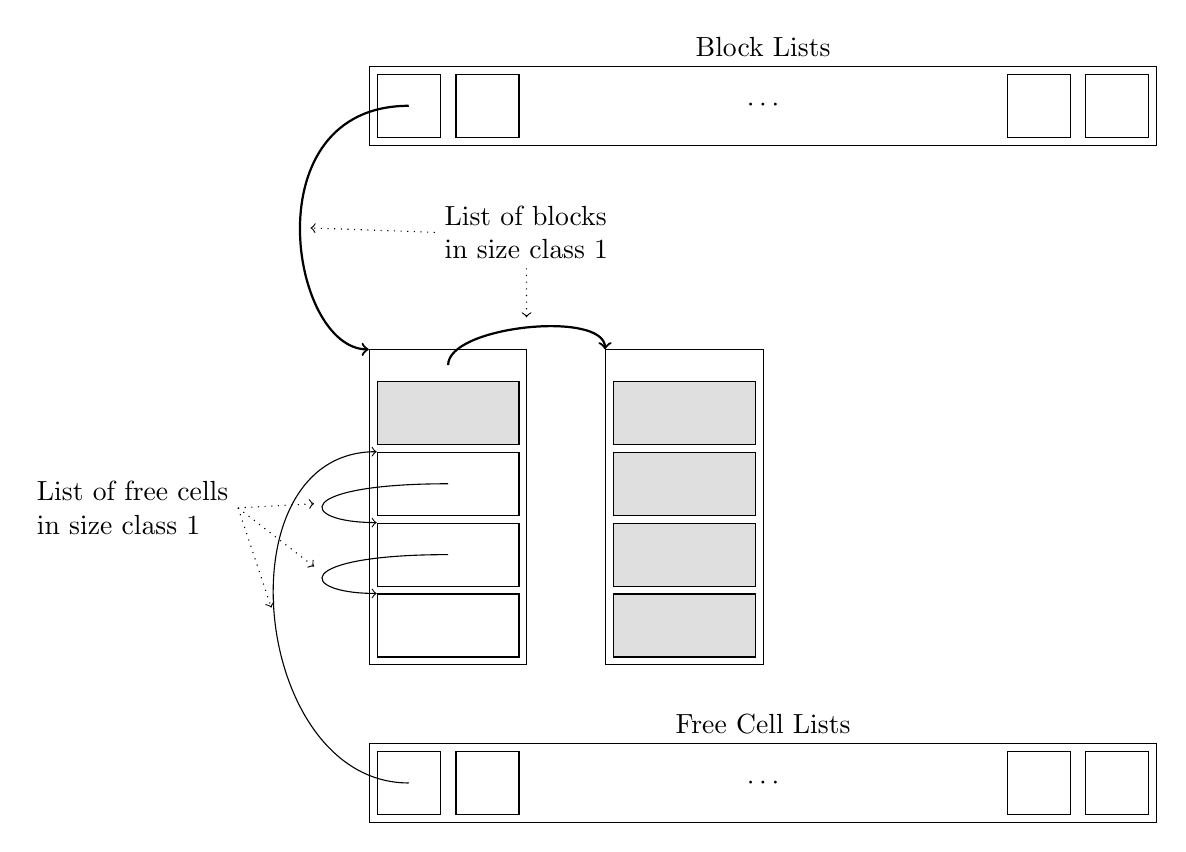
\begin{tikzpicture}



\newcommand*{\heads}[1]{
\draw (0,0) node [draw,shape=rectangle,minimum width=10cm,minimum height=1cm,
                      anchor=south west]
            (#1) {$\cdots$};

 \draw (0.1,0.1) node [draw,shape=rectangle,minimum width=8mm,minimum
height=8mm, anchor=south west] (#1-1) {}; 
\draw (1.1,0.1) node [draw,shape=rectangle,minimum width=8mm,minimum height=8mm,
                      anchor=south west] {}; 

\draw (8.1,0.1) node [draw,shape=rectangle,minimum width=8mm,minimum height=8mm,
                      anchor=south west] {}; 
\draw (9.1,0.1) node [draw,shape=rectangle,minimum width=8mm,minimum height=8mm,
                      anchor=south west] {}; 
}

\tikzstyle {block}=[draw,shape=rectangle,
     minimum width=20mm,minimum height=40mm, anchor=south west];

\tikzstyle {cell}=[draw,shape=rectangle,
     minimum width=18mm,minimum height=8mm, anchor=south west];

\tikzstyle {object}=[cell, fill=gray!25];


\begin{scope}[yshift=9.6cm]
\heads{bps}
\draw (bps.north) node [above] {Block Lists};
\end{scope}
\begin{scope}[yshift=1cm]
\heads{cps}
\draw (cps.north) node [above] {Free Cell Lists};
\end{scope}



\begin{scope}[yshift=3cm]
%\draw (0,0)  -- ++(0,4) -- ++(2,0) -- ++(0,-4) -- ++(-2,0);
\draw (0,0) node [block] (b1) {};
\draw (0.1,0.1) node [cell] (o14) {};
\draw (0.1,1.0) node [cell] (o13) {};
\draw (0.1,1.9) node [cell] (o12) {};
\draw (0.1,2.8) node [object] (o11) {};
\end{scope}

\begin{scope}[yshift=3cm, xshift=3cm]
%\draw (0,0)  -- ++(0,4) -- ++(2,0) -- ++(0,-4) -- ++(-2,0);
\draw (0,0) node [block] (b2) {};
\draw (0.1,0.1) node [object] (o24) {};
\draw (0.1,1.0) node [object] (o23) {};
\draw (0.1,1.9) node [object] (o22) {};
\draw (0.1,2.8) node [object] (o21) {};
\end{scope}

% List of blocks
\draw [->,thick] (bps-1.center) .. controls +(left:2cm) and +(left:1cm) .. 
           node (bp1) {}
           (b1.north west);

\draw [->,thick] (b1.north)+(0,-2mm) .. controls +(up:5mm) and +(up:5mm) ..
           node (bp2) {}
           (b2.north west);

% List of cells
\draw [->] (cps-1.center) .. controls +(left:2cm) and +(left:2cm) .. 
           node (cp1) {}
           (o12.north west);

\draw [->] (o12.center) .. controls +(left:2cm) and +(left:1cm) ..  
           node (cp2) {}
           (o13.north west); 

\draw [->] (o13.center) .. controls +(left:2cm) and +(left:1cm) .. 
           node (cp3) {}
           (o14.north west); 

% Labels of free list pointers
\draw (-3,5) node [minimum width=20mm,align=left] (fltext)
  { List of free cells\\in size class 1 };
  
\draw [->,dotted] (fltext.east) -- (cp1);
\draw [->,dotted] (fltext.east) -- (cp2);
\draw [->,dotted] (fltext.east) -- (cp3);

% Labels of block list pointers
\draw (2,8.5) node [minimum width=20mm,align=left] (bltext)
  { List of blocks\\in size class 1 };
  
\draw [->,dotted] (bltext.west) -- (bp1);
\draw [->,dotted] (bltext) -- (bp2);
\end{tikzpicture} 
\end{center}
\caption{Blocks and cells in the segregated free list}
\end{figure}

\section{Lazy Sweeping}
\label{sec:ms:lazy}



\section{Mark-state implementation}
\label{sec:ms:state}




\begin{lstlisting}[name=Mark Phase, 
                   caption=\lstname: pseudo-code for mark-sweep,
                   label=fig:ms:pseudo]
                   
work.addAll(root-set)
for (obj = work.pop(); obj != null;obj = work.pop() ) {
  for (ref : obj.references()) {
    if (ref != null && ref.get().testAndMark()) {
      work.push(ref.get())
    }
  }
}
\end{lstlisting}



% Generational Collection
\input{generational}

% Concurrency
\input{concurrent}

% Complications, Language Features
\input{features}

\part{Mechanisms}

\input{plans}

% Plans.  Stop-the-world. Generational. Reference Counting. Concurrent.

% Policies: Spaces
\chapter{Policies}

\section{Large Object Space}
\label{sec:policy:LargeObject}
% Virtual memory management

% Queues

% VM Interface(s)

\part{Implementations}

\chapter{Allocators}
\section{Segregated Free List}
\label{sec:alloc:free-list}

\section{Bump Pointer}
\label{sec:alloc:bump-pointer}



% The MMTk Harness

% Jikes RVM

\chapter*{References}

\bibliographystyle{plainnat}
\bibliography{mmtk-guide}




\end{document}
